\graphicspath{{chapters/vuvuzela/images/}}
\chapter{Updates to the Noise Simulation}
\label{chapter:vuvuzela}
The search for tau neutrinos is a search for events near the detector threshold.
Under these conditions, the search requires excellent understanding of threshold effects and detector behavior.
In order to better model the detector, the noise simulation used in IceCube was updated with improved measurements after the discovery of disagreements in charge variables.
This process is described in this chapter.

The chapter begins by describing the process used previously to fit the Vuvuzela noise model for each DOM.
The limitations of the previous fitting process and the discovery of new disagreements is discussed in Sections~\ref{sec:vuvuzela_limitations} and \ref{sec:lowdt_vuvuzela} respectively.
The new fitting procedure is then described in Section~\ref{sec:vuvuzela_fitting}.
New results of the fitting procedure are then discussed in Section~\ref{sec:vuvuzela_newfits}.

\section{A Summary of Previous Fits}
\label{sec:old_vuvuzela}
Detector noise is a nuisance in most physics and astronomy experiments.
PMT noise is assumed to be due to random emission of electrons from the photocathode and is affected by the gain of the PMT.

A purely Poissonian noise model was used in the past in IceCube. 
With the introduction of the looser SMT3 trigger in DeepCore in 2010 it became clear that additional unsimulated sources of noise exist \cite{Thesis-Vuvuzela}.
These additional photoelectrons appeared to occur in 'bursts' on a single DOM extending for up to a millisecond.
Due to the time-correlations of these emitted photons, the phenomenon was labeled \emph{correlated noise}.

The Vuvuzela model, described briefly in Section~\ref{subsec:noise}, is now used to model both the Poissonian and non-Poissonian noise in IceCube.
The empirical model consists of a Poisson process for electronic noise and radioactive decays and a correlated component modeled with a log-normal distribution.
The model contains five free parameters per DOM.
Ten minutes of untriggered data from the detector, dominated by noise hits, was used for calibration of the Vuvuzela parameters.

The Vuvuzela noise model is fit using the distributions of the time between subsequent hits, shown previously in Figure~\ref{fig:noise_model}.
Fits for each DOM were performed using the Pearson chi-squared test statistic between the data histogram, $d$, and the simulated histogram, $m$.

\begin{equation}
\chi^2 = \sum_i^{bins} \frac{\left(d_i-m_i\right)^2}{m_i}
\end{equation}

\begin{figure}[h]
\centering
\begin{tabular}[b]{c}
  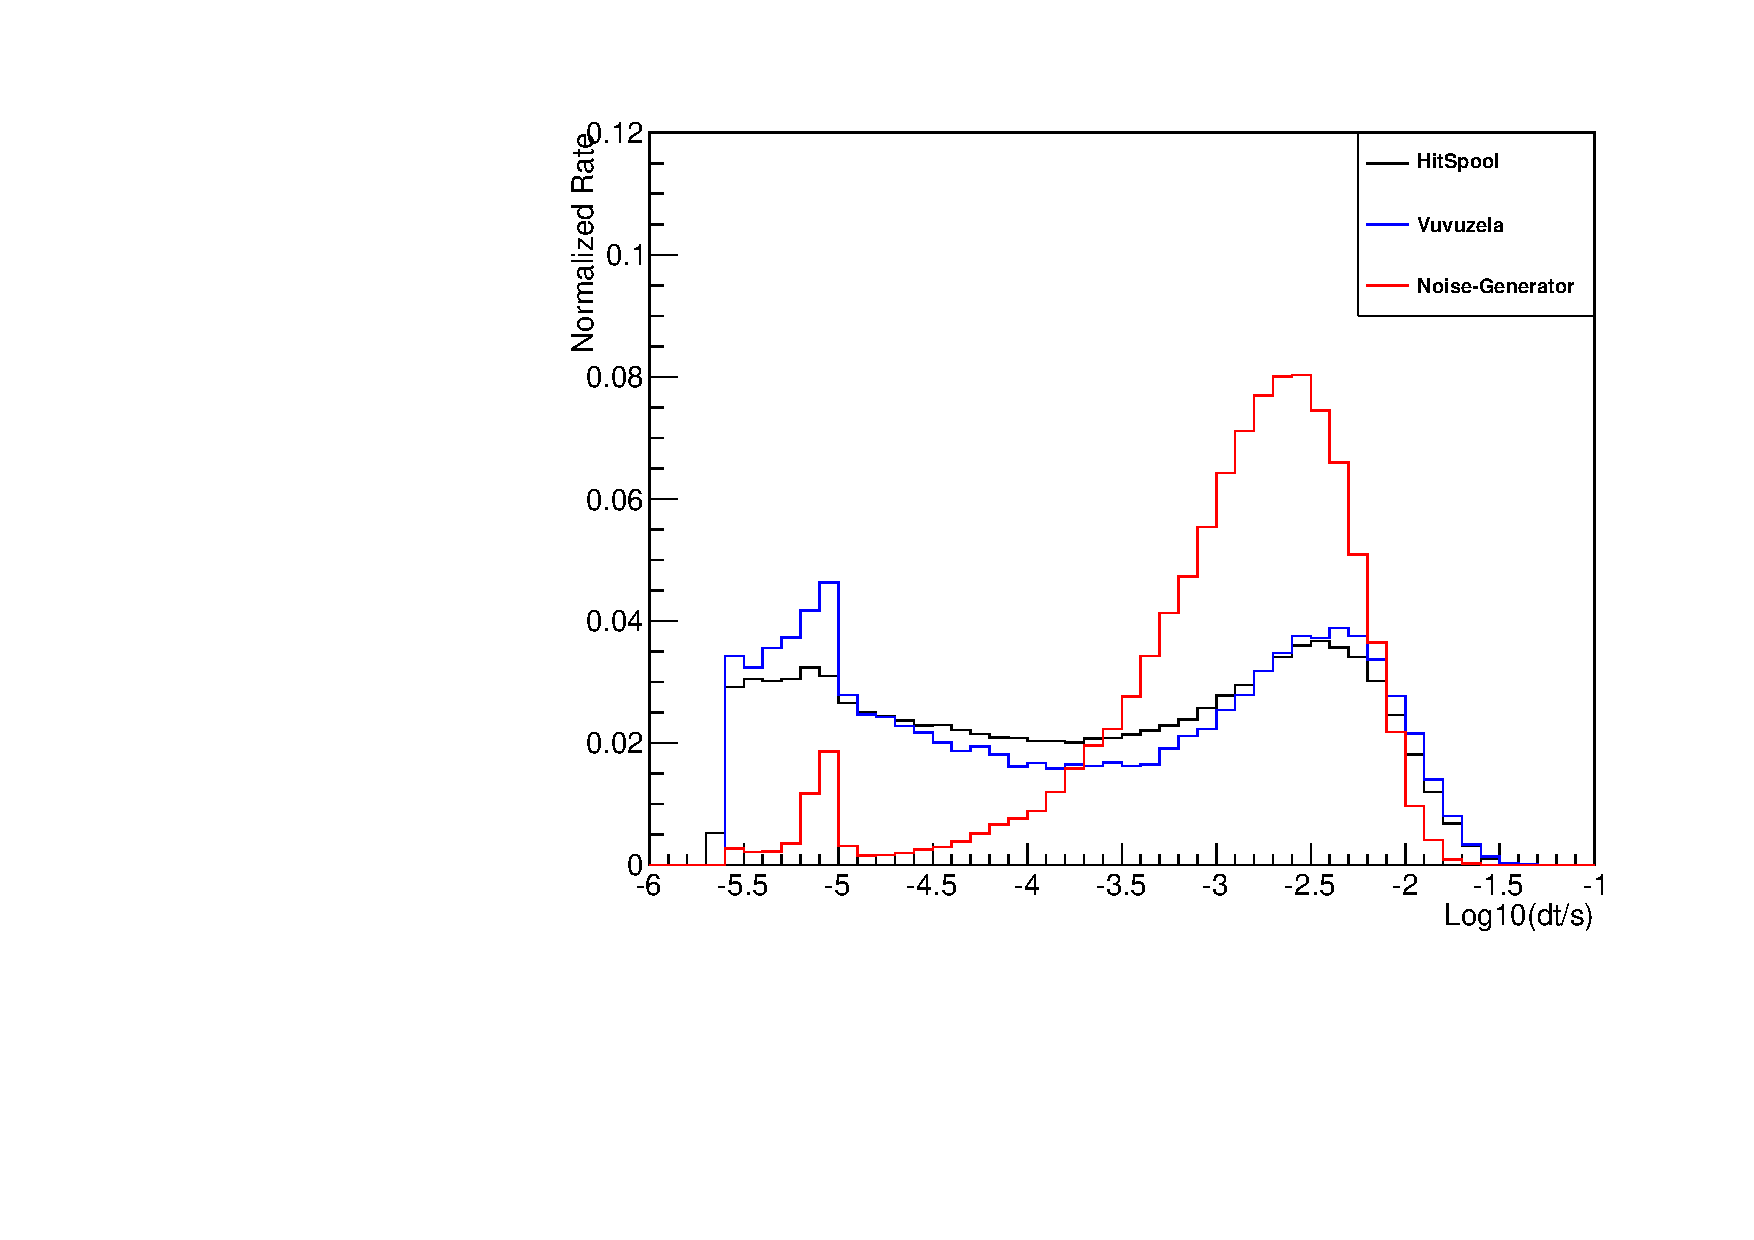
\includegraphics[width=0.45\linewidth]{old_dom_11-19.pdf} \\
  \small (\textbf{\color{ctcolormain}a}) DOM 11-19
\end{tabular} \hspace{2pt}
\begin{tabular}[b]{c}
  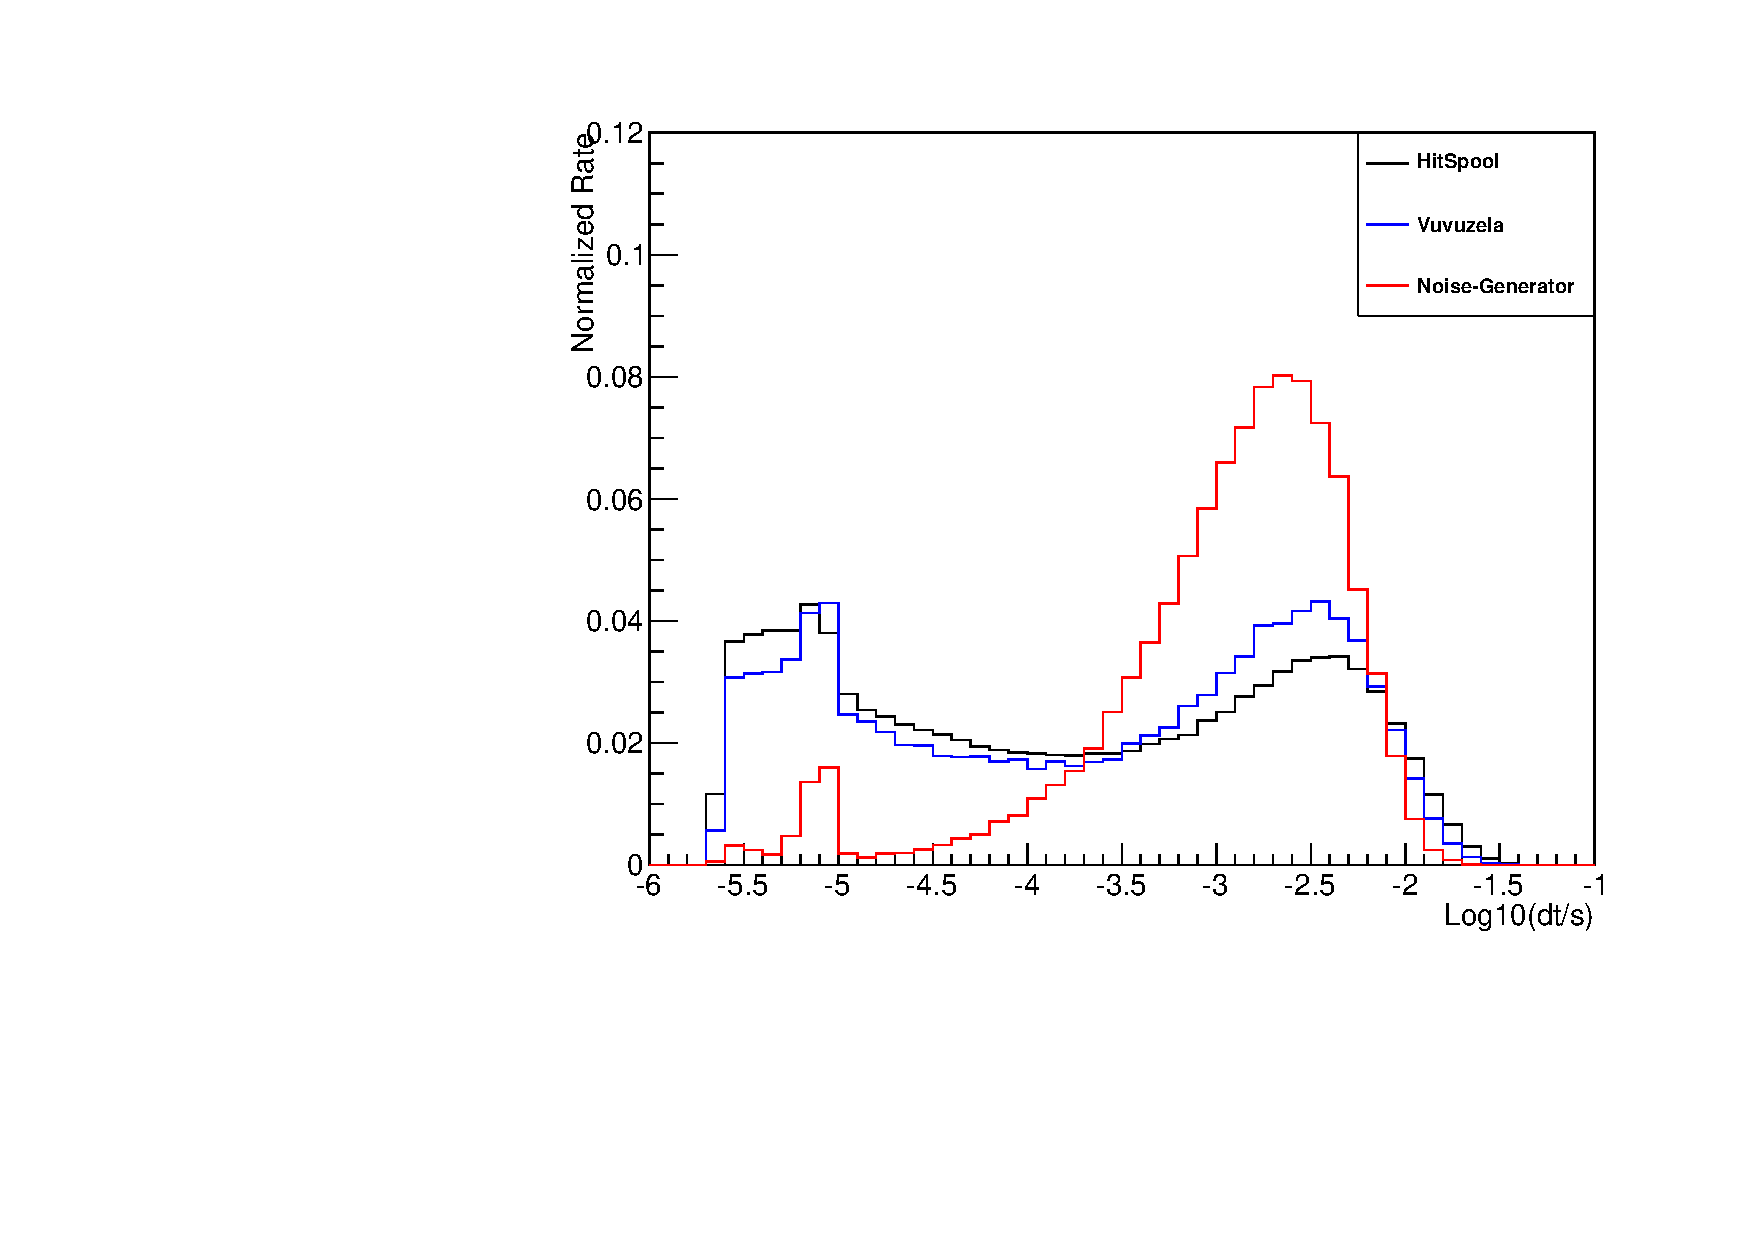
\includegraphics[width=0.45\linewidth]{old_dom_83-42.pdf} \\
  \small (\textbf{\color{ctcolormain}b}) DOM 83-42
\end{tabular}
\caption[Examples of noise distributions from Vuvuzela V1 calibrations]{Two examples of the original calibration work for the Vuvuzela noise model. The x-axis measures the time between consecutive hits on a single DOM ("dt"). Untriggered detector data is given by the black line. In red, a purely Poissonian noise model is shown. An afterpulsing peak is visible at $10^{-5}$ s. The Vuvuzela mode, in blue,l shows better agreement than the purely Poissonian noise model at all timescales.}
\label{fig:old_vuvuzela_fits}
\end{figure}


The value of the $\chi^2$ was minimized using a Metropolis-Hastings algorithm \cite{PDG-2015}.
For each iteration of the algorithm, new parameters were selected and the response of the DOM was resimulated using PMTResponseSimulator and DOMLauncher.
Each fit was computationally intensive, requiring between two and four CPU-weeks for each DOM.
Due to the computational requirements of the fits, the stopping condition was intentionally loosely defined, with a goodness-of-fit of 10\% used.

\begin{figure}
\centering
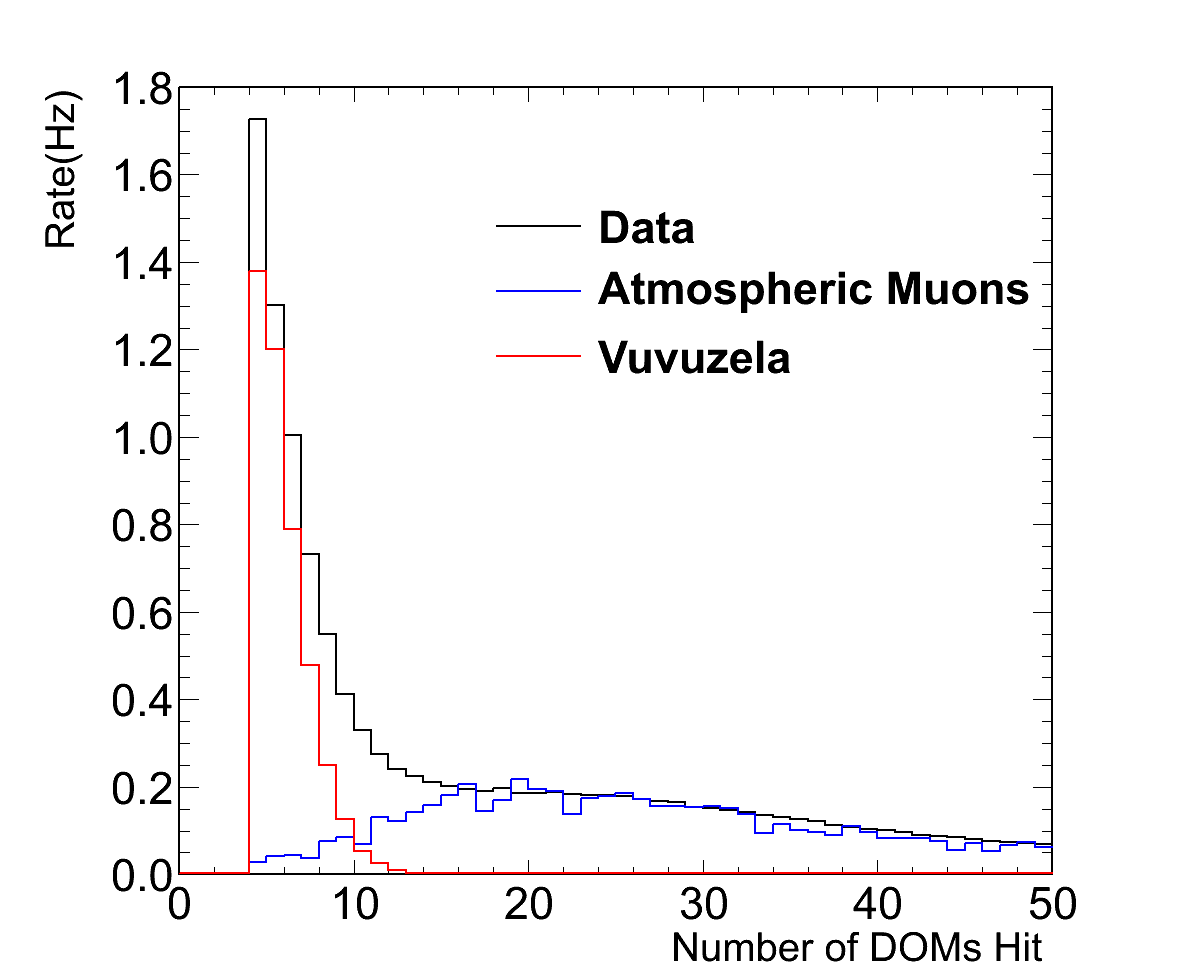
\includegraphics[width=0.6\textwidth]{srtwofflinepulsesdc_withnoise_vuvuzela.png} 
\caption[Noise trigger rates with Vuvuzela V1]{The rates of events in DeepCore as a function of the number of hit DOMs in a cleaned hit series. The data, shown in black, consists of two components: the accidental triggers (red) and the atmospheric muons (blue). Accidental triggers produced using the Vuvuzela noise model reproduce most of the rate of events below 10 hit DOMs, although a rate disagreement remains. Image from \cite{Thesis-Vuvuzela}.}
\label{fig:old_nch}
\end{figure}

Two examples from the original calibration work are shown in Figure~\ref{fig:old_vuvuzela_fits}.
The Poissonian noise model used previously is shown for comparison.
The Vuvuzela model more accurately reproduces the observed data across all timescales than the purely Poissonian noise model used in the past.
Distributions of the number of hit DOMs and the number of accidental triggers due to detector noise, shown in Figure~\ref{fig:old_nch}, improve significantly after inclusion of the updated noise model \cite{Thesis-Vuvuzela}.

\section{Limitations and Disagreement with Previous Fits}
\label{sec:vuvuzela_limitations}
While accidental triggers with the Vuvuzela model better reproduced the rates observed in data, Figure~\ref{fig:old_nch} showed disagreement between data and simulation at very low numbers of hits.
This region of the parameter space is dominated by accidental noise triggers in simulation.

An evaluation of the previous calibration was performed in 2014, uncovering a number of possible improvements related to various modeling assumptions or omissions.
For example, the original Vuvuzela fits excluded the effect of atmospheric muons in the detector under the assumption that the hit rate per DOM due to atmospheric muons (approximately 5 Hz) is significantly smaller than the noise hit rate observed in previous calibration (about 600 Hz).
Potential issues may arise from this assumption, which was not tested during original calibrations, including any potential time-correlated hits associated with muons.

Furthermore, some fits resulted in potentially-incomplete minimization.
Due to the nature of the fit distributions, there existed significant degeneracy in the parameter space, leading to further difficulties.

During the fitting process, the strength of the afterpulsing peak at 9 microseconds was discovered to differ between DOMs.
This effect was unsimulated, leading to convergence problems when fitting this region.
In response, fits were artificially limited to timescales longer than 10 microseconds, allowing the minimizer to only observe part of the correlated noise distribution.

Because the noise hits are unlikely to satisfy the HLC conditions, timescales smaller than 6.4 microseconds were unavailable for investigation.
No checks were performed for the Vuvuzela model below this limit.
However, the noise model was used down to 2 microseconds resulting in uncertainty due to the extrapolation to shorter times.
The limit of 2 microseconds was implemented due to the inherent difficulty in characterizing effects at these timescales due to artificial deadtime related to the HLC launch readout. 

\section{Low-dt Noise from Vuvuzela}
\label{sec:lowdt_vuvuzela}
In an attempt to address the imposed simulation limit at 2 microseconds, a new version of the Vuvuzela code was created with this cutoff removed.
The resulting noise, labeled \emph{low-dt} noise for the short timescales ($\Delta$t), was used to produce a simulation of accidental noise triggers and CORSIKA muons for testing without further calibration.

\begin{figure}[h]
\centering
\begin{tabular}[b]{c}
  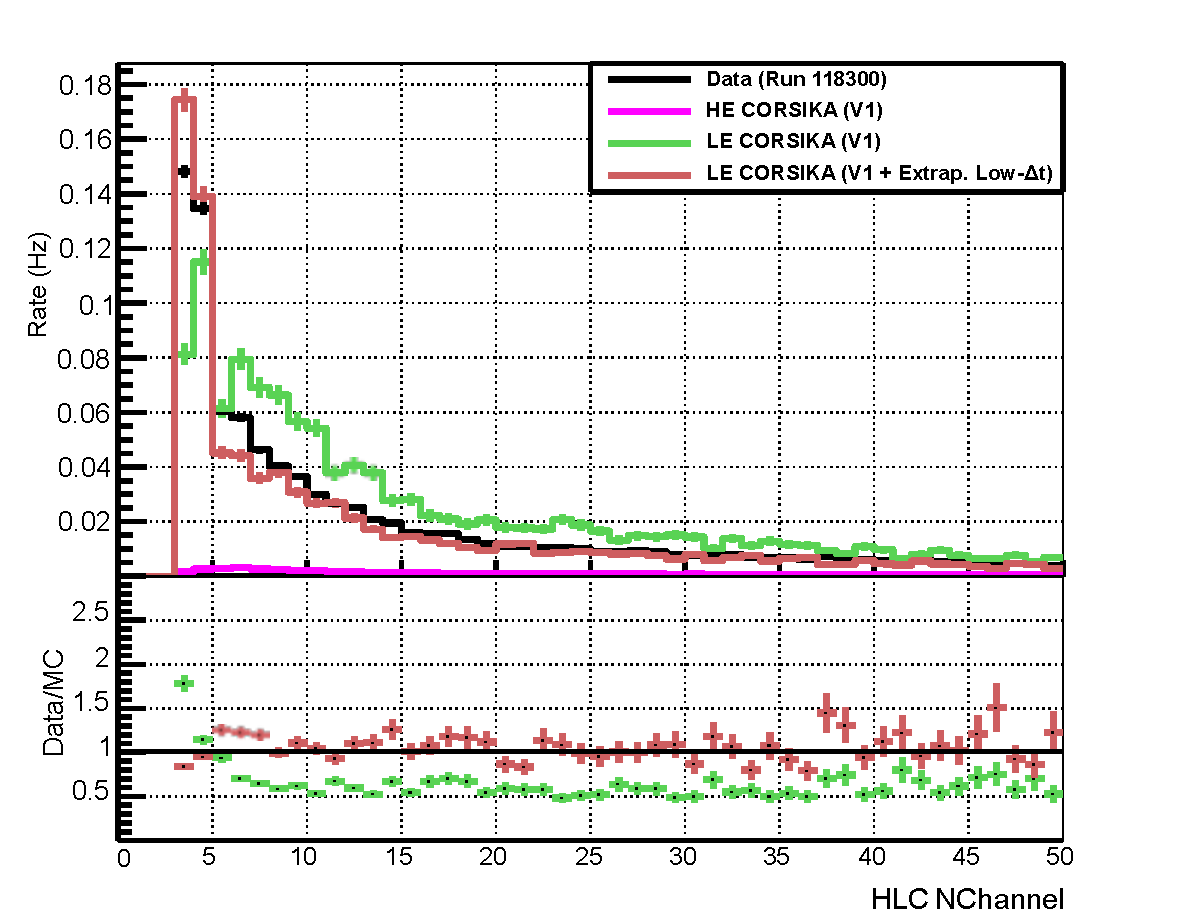
\includegraphics[width=0.45\linewidth]{old_HLC_NChannel.pdf} \\
  \small (\textbf{\color{ctcolormain}a}) HLC hits in DeepCore Events
\end{tabular} \hspace{2pt}
\begin{tabular}[b]{c}
  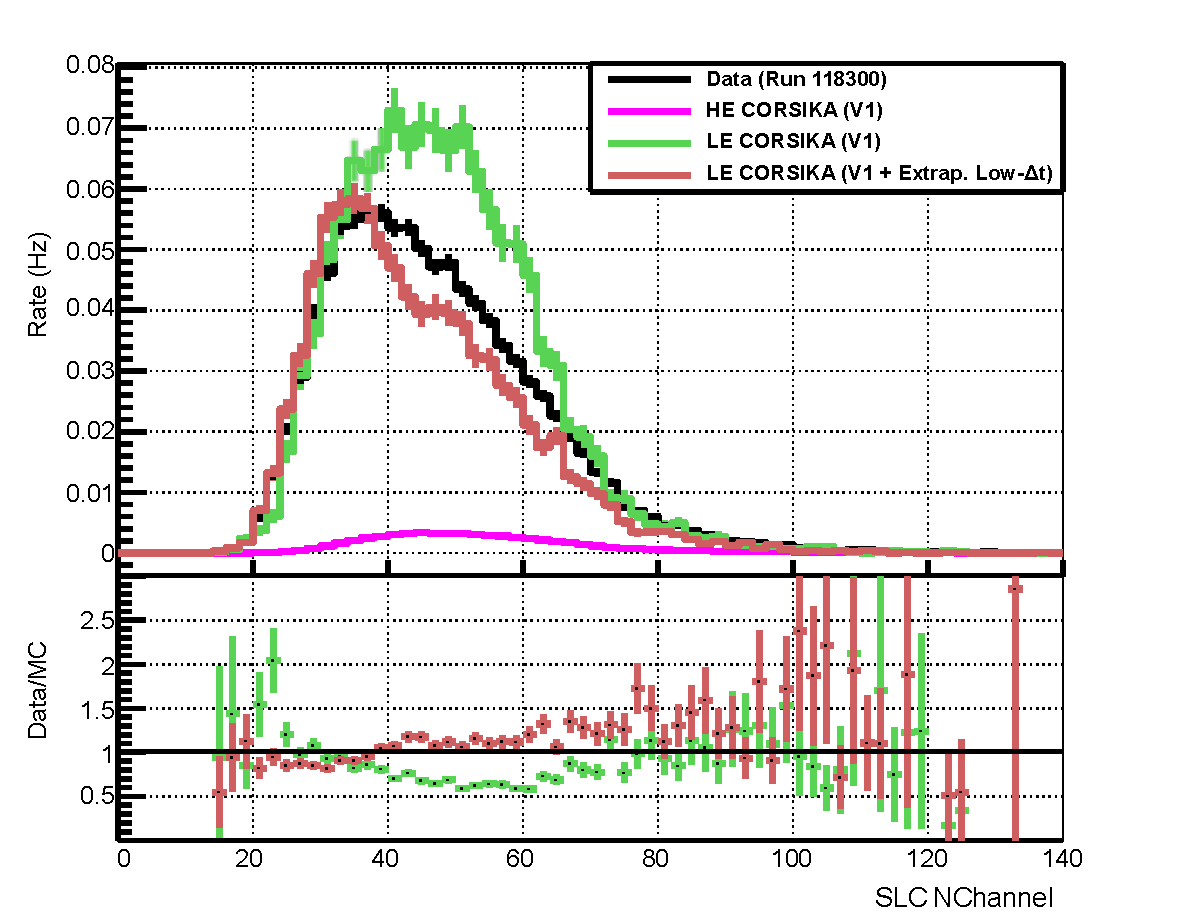
\includegraphics[width=0.45\linewidth]{old_SLC_NChannel.pdf} \\
  \small (\textbf{\color{ctcolormain}b}) SLC hits in DeepCore Events
\end{tabular}
\caption[HLC and SLC number of hit DOMs with Vuvuzela V1]{The number of hit DOMs satisfying the (a) HLC and (b) SLC criteria described in Section~\ref{subsec:LC}. The distribution from 8 hours of data (black) is shown compared to a sample of CORSIKA muons at low-energy (600 GeV $\leq E_{primary} \leq$ 100 TeV) and high energy (100 TeV $\leq E_{primary} \leq$ 100 EeV). The addition of the low-dt extension to Vuvuzela improves the agreement between data and simulation in both HLC and SLC distributions.}
\label{fig:uncalibrated_nchannel}
\end{figure}

The first tests, shown in Figure~\ref{fig:uncalibrated_nchannel}, used the number of hit DOMs in DeepCore events to evaluate the effect of the low-dt noise extension.
The number of accidental triggers, dominant for events with fewer than 5 HLC hits, increased with the additional noise hits.
The number of muons, which make up the majority of events with more than 10 HLC hits, decreased due to the use of the DeepCoreFilter, a veto described in further detail in Section~\ref{sec:DeepCoreFilter}.
Both effects led to improved agreement between data and simulation.

\begin{figure}[h]
\centering
\begin{tabular}[b]{c}
  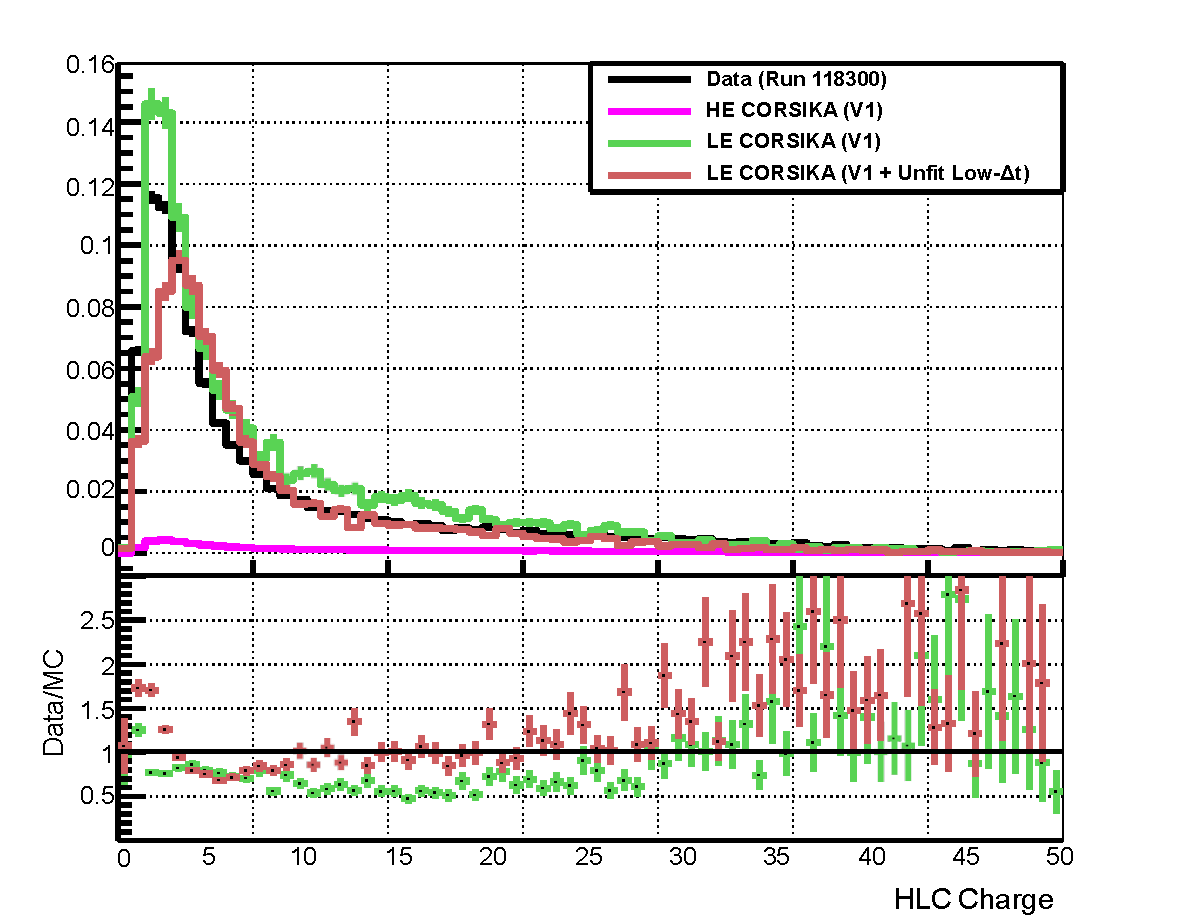
\includegraphics[width=0.45\linewidth]{old_HLC_Charge.pdf} \\
  \small (\textbf{\color{ctcolormain}a}) HLC Charge in DeepCore Events
\end{tabular} \hspace{2pt}
\begin{tabular}[b]{c}
  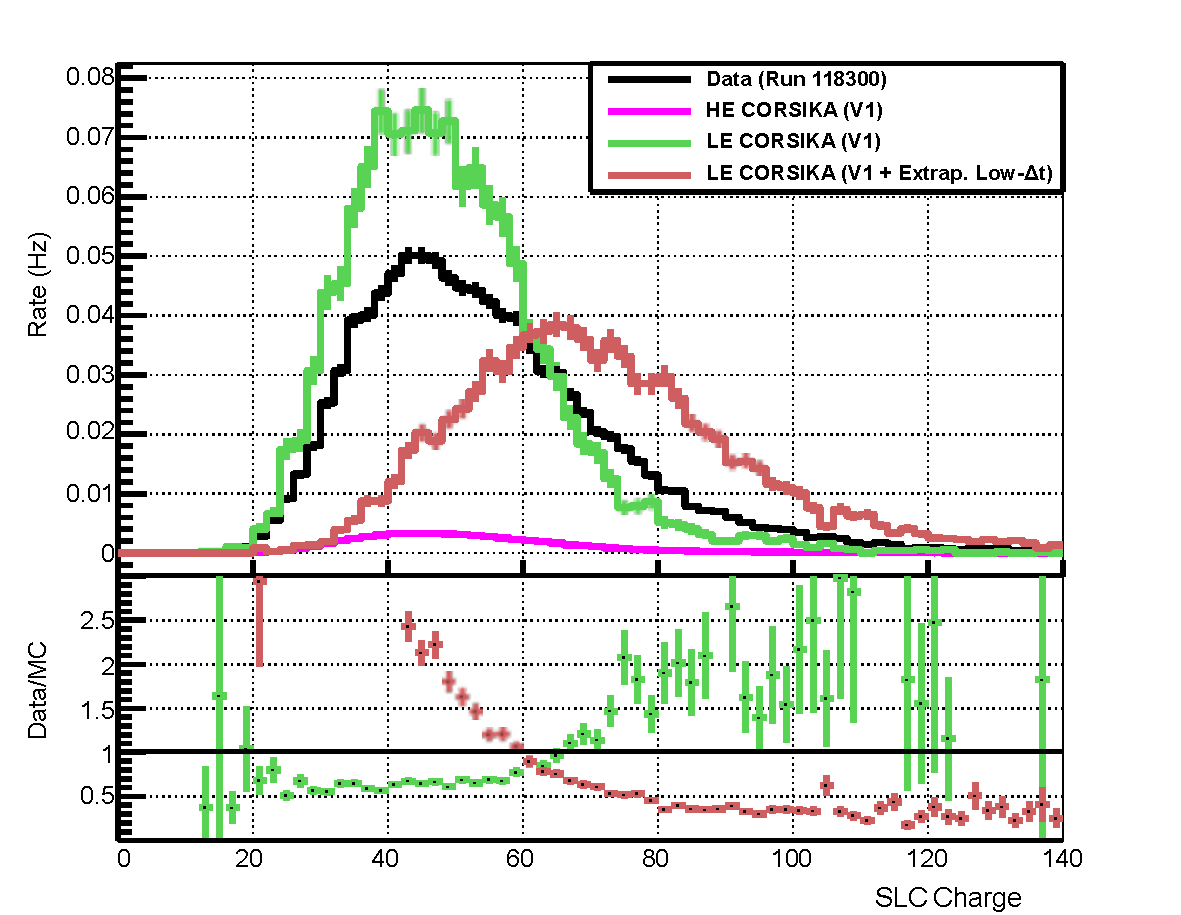
\includegraphics[width=0.45\linewidth]{old_SLC_Charge.pdf} \\
  \small (\textbf{\color{ctcolormain}b}) SLC Charge in DeepCore Events
\end{tabular}
\caption[HLC and SLC charge with Vuvuzela V1]{The total amount of charge on DOMs satisfying the (a) HLC and (b) SLC criteria described in Section~\ref{subsec:LC}. The distribution from 8 hours of data (black) is shown compared to a sample of CORSIKA muons at low-energy (600 GeV $\leq E_{CR} \leq$ 100 TeV) and high energy (100 TeV $\leq E_{CR} \leq$ 100 EeV). Unlike in Figure~\ref{fig:uncalibrated_nchannel}, the charge distributions using the low-dt extension to Vuvuzela shows large disagreements with data. This is most visible in the SLC charge distribution.}
\label{fig:uncalibrated_charge}
\end{figure}

Because the extended noise model adds hits occuring at timescales down to nanoseconds, multiple hits can occur within one waveform, leading to increased observed charge.
When the noise distribution is extended below 2 microseconds, the tail of the distribution falls into the ATWD window of 322 nanoseconds, increasing the charge of noise hits in HLC DOMs.
Furthermore, some fraction of the hits in a burst of correlated noise occur within the three bins recorded from the FADC for SLC hits.
The result is that SLC hits at the start of a noise may appear as an integration of multiple single pulses.
Such an effect would be most visible in the charge distribution of SLC DOMs, which are more likely to be due to noise hits than HLC DOMs.

The total charge of DOMs associated with HLC and SLC hits was evaluated to look for this effect due to the extended noise model.
The result is shown in Figure~\ref{fig:uncalibrated_charge}.
The change in the charge is observed clearly in the SLC charge distribution, where a systematic shift is visible due to the low-dt extension.
Both the original Vuvuzela model and the extended Vuvuzela model show significant disagreement with data in the SLC charge distribution.
The strong effect and continuing disagreement in the SLC charge distribution with data demonstrated that the noise distribution at very short timescales was an important effect that deserved further attention.

\begin{figure}[h]
\centering
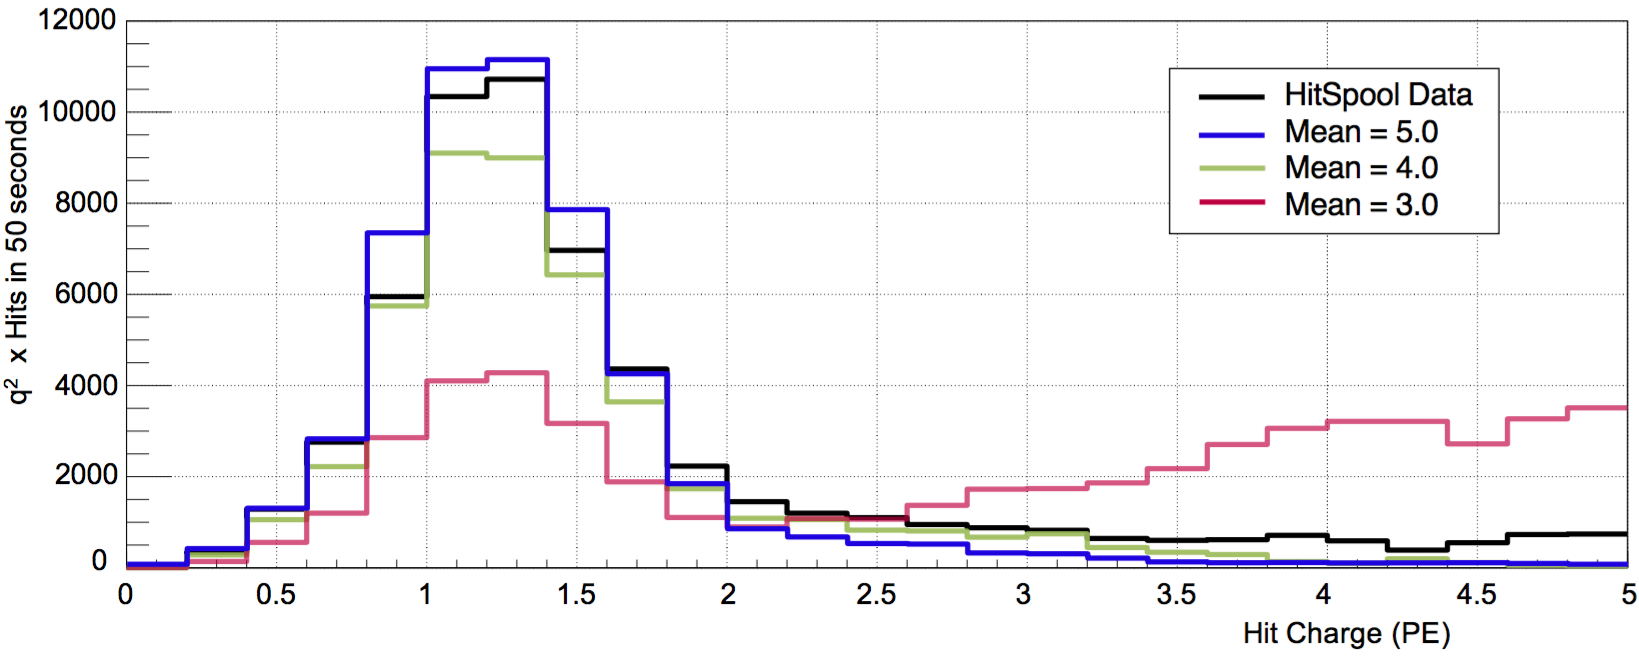
\includegraphics[width=0.5\pagewidth]{lowdt_charge_effects.png} 
\caption[The effect of low-dt Vuvuzela in the charge distribution]{The effect of changing the Vuvuzela noise model parameters on the charge distribution of observed launches. Note the scale of the y-axis, which is scaled in order to emphasize the effect. Here, the gaussian mean is shifted from "5" (100 microseconds) to "3" (1 microsecond). All other parameters are held constant. By moving the correlated noise distribution to shorter timescales, more of distribution falls into one FADC bin, increasing the charge output for each launch. }
\label{fig:lowdt_effect_charge}
\end{figure}

The observed effect of the low-dt extension on the SLC charge distribution indicates that the distribution is sensitive to the region below 2 microseconds.
The charge distribution of each DOM may therefore be used in the fitting procedure in order to characterize the low-dt end of the noise timing distribution.
The effect, demonstrated in Figure~\ref{fig:lowdt_effect_charge}, allows the investigation of a part of the distribution unavailable in previous fits.

\section{Updating the Fitting Code}
\label{sec:vuvuzela_fitting}
The effect of the low-dt extension on the charge distributions indicated the potential for improvement in the noise model distribution.
New calibration fits for the updated the noise model, referred to as \emph{Vuvuzela V2} fits, were planned to include this extension for all DOMs.

With the opportunity to refit, a number of additional improvements were implemented.
The afterpulsing peak at 9 microseconds was explicitly included in the fitting code.
To account for the variability in the strength of the peak, a scale factor for the afterpulsing was included in the Vuvuzela V2 fits.

In order to include the effect of atmospheric muons, a set of Polygonato CORSIKA.
The Polygonato model was selected due to the natural weighting scheme of the output files, allowing continuous simulation of the detector.
Simulated files were divided into 10 microsecond long events (\emph{long-frame} events), each containing multiple muons.
The simulation was halted after photon propagation, giving a collection of muons without detector noise and effects applied.

\begin{landscape}
\centering
\begin{figure}
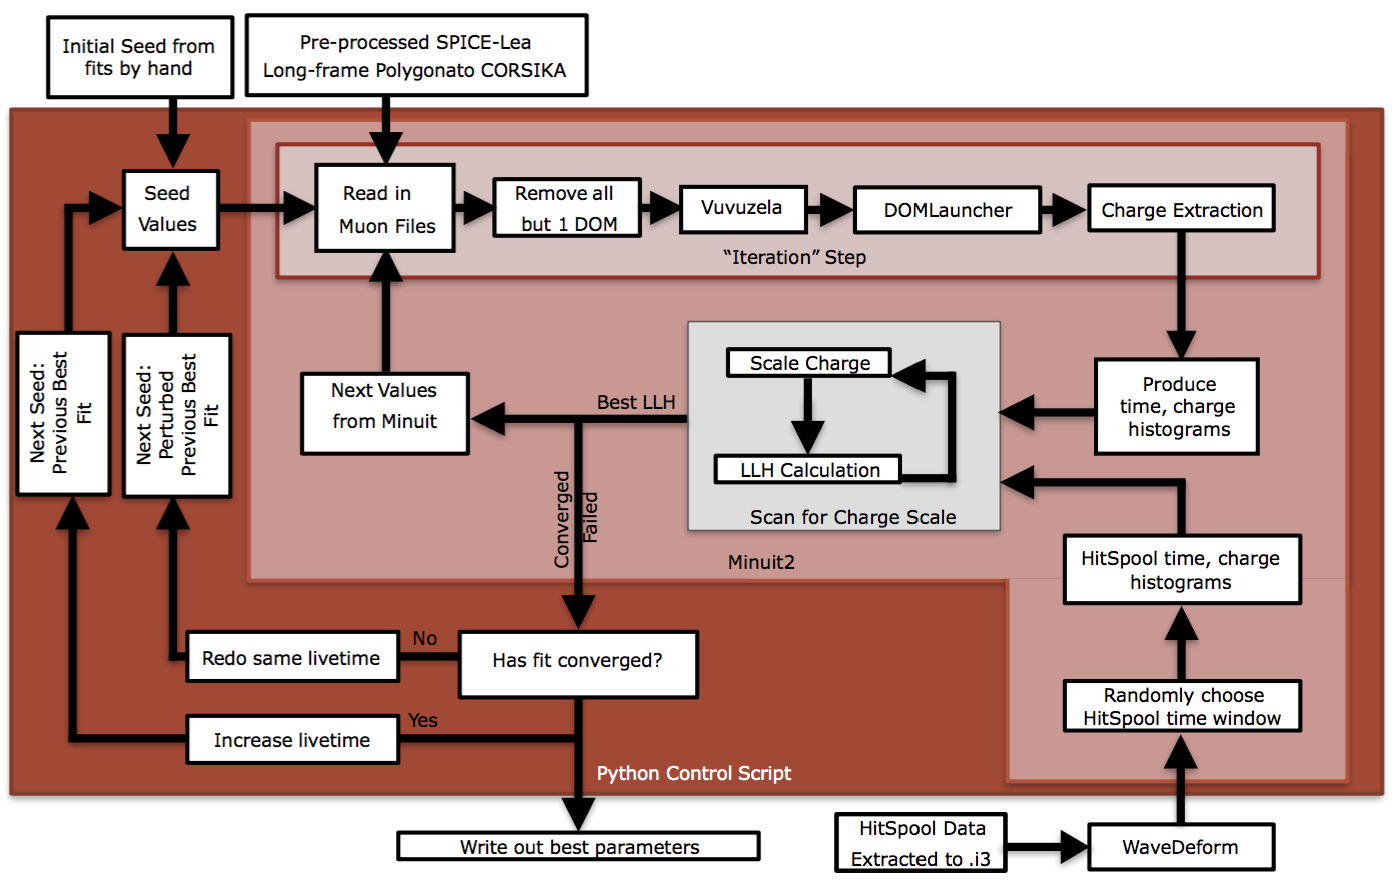
\includegraphics[height=0.8\textwidth]{fit_flowchart.png} 
\caption[Schematic diagram of Vuvuzela V2 calibration fit]{A schematic diagram of the process used in the Vuvuzela V2 calibration fit.}
\label{fig:fit_flowchart}
\end{figure}
\end{landscape}

The fitting process, described schematically in Figure~\ref{fig:fit_flowchart}, is divided into several parts. 
The code started with untriggered detector data as well as the produced long-frame CORSIKA events. 
The fit included a total of six explicit parameters: the five parameters from the original Vuvuzela model as well as a scale factor for the afterpulsing.
Later investigations led to the introduction of a charge scale parameter to account for systematic differences between the data and simulated charge.
Seeds for each parameter were taken from the Vuvuzela V1 calibration fits from 2012.
Fits were performed for each DOM in parallel.

For each iteration, the long-frame CORSIKA files were filtered to remove information on all DOMs not currently being fit in order to limit the processing power required for DOM simulation.
The noise and detector simulation were applied using the current parameter set for the iteration.
Charge extraction from the waveforms was performed using standard IceCube tools.
After the simulation for a given set of parameters, histograms were produced for untriggered data and simulated launches.
As in the previous fits, the time between subsequent hits is used as the primary observable of the noise behavior.
In addition, the observed charge on the DOM is used as a second observable for new fits.

\begin{figure}[h]
\centering
\begin{tabular}[b]{c}
  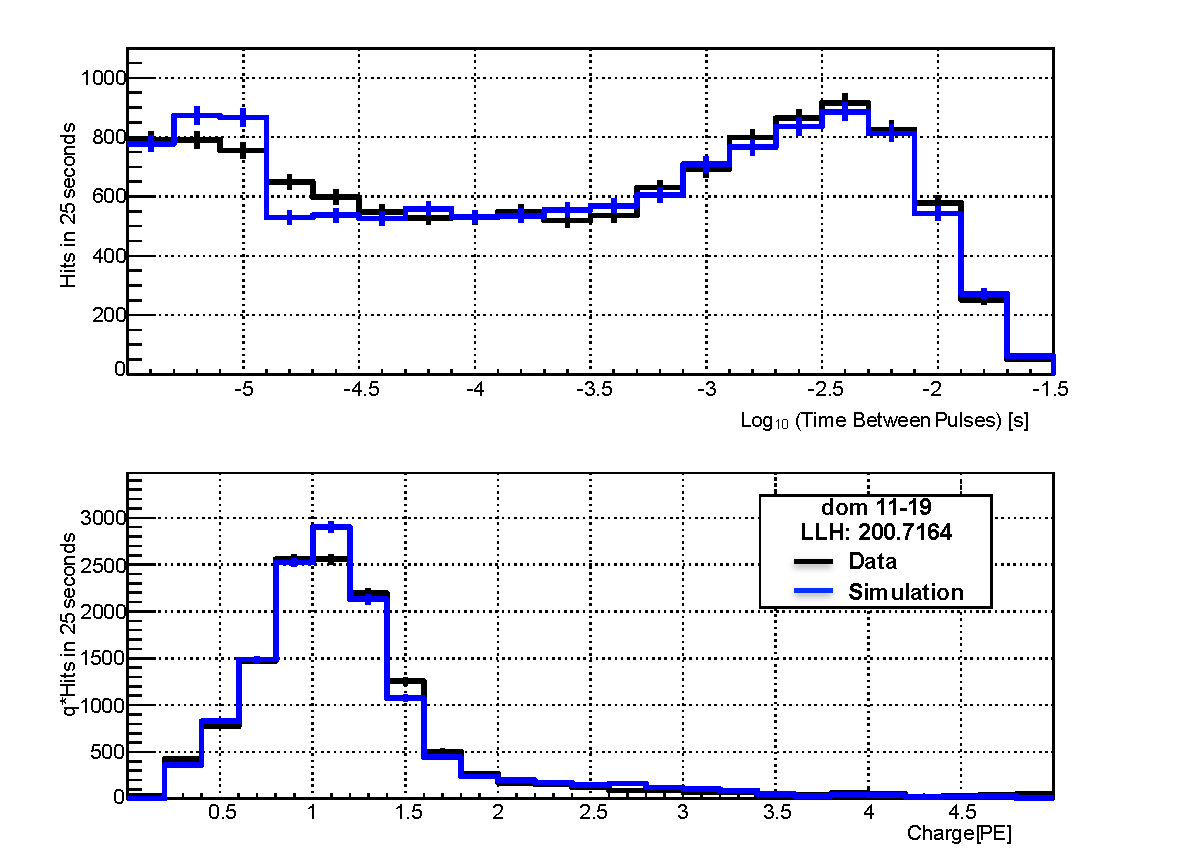
\includegraphics[width=0.45\linewidth]{new_dom_11-19.pdf} \\
  \small (\textbf{\color{ctcolormain}a}) DOM 11-19
\end{tabular} \hspace{2pt}
\begin{tabular}[b]{c}
  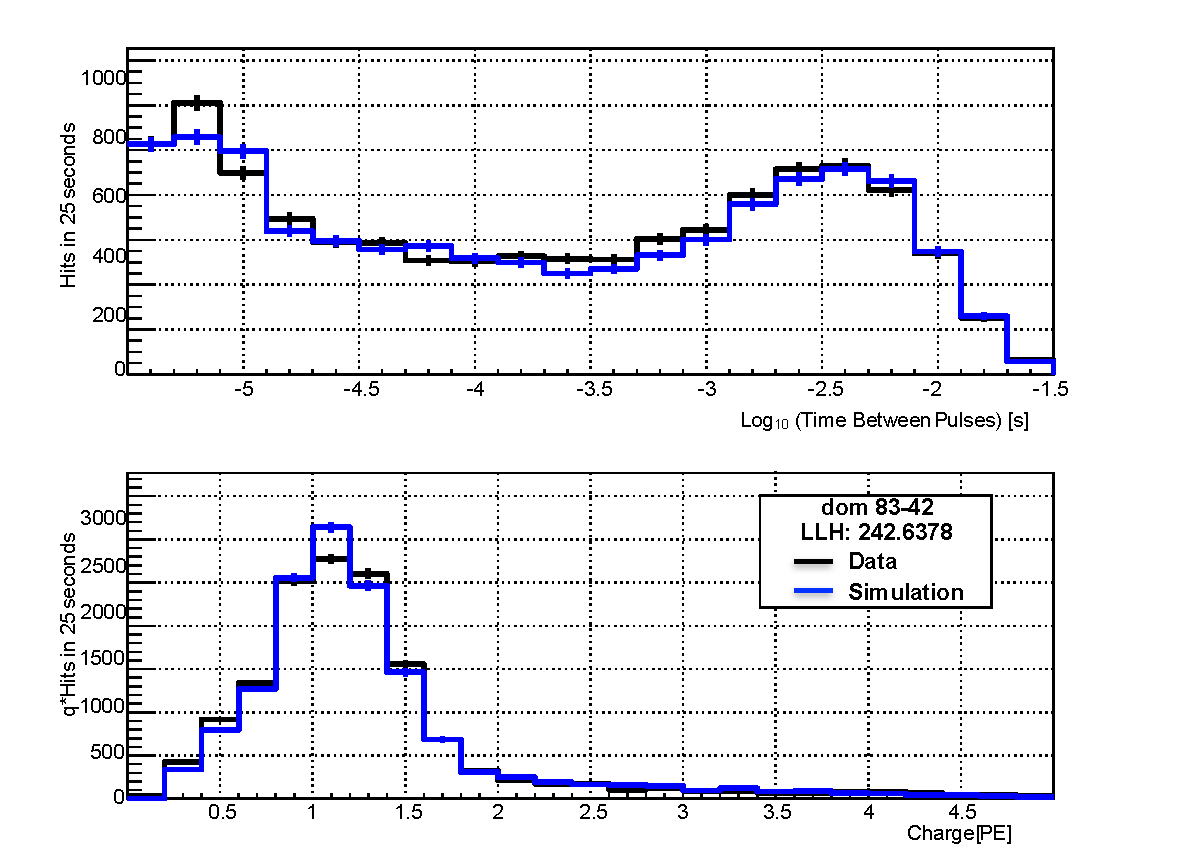
\includegraphics[width=0.45\linewidth]{new_dom_83-42.pdf} \\
  \small (\textbf{\color{ctcolormain}b}) DOM 83-42
\end{tabular}
\caption[Examples of Vuvuzela V2 noise fits]{Two examples of the new calibration fits for the Vuvuzela V2 model. The distribution of the time ("dt") between hits and the distribution of charge per launch are shown on top and bottom respectively.The untriggered data, in back, is compared to the Vuvuzela V2 model in blue. The new fits shown good agreement in both time and charge distributions. Note that the y-axis of the charge distribution is scaled by the charge value.}
\label{fig:new_vuvuzela_fits}
\end{figure}

The timing histogram is binned from 6 microseconds until 1 second.
Short timescales are measured through the effect on the charge distributions, which are binned from 0 to 5 PE in charge.
The distributions for DOMs 11-19 and 83-42 are shown in Figure~\ref{fig:new_vuvuzela_fits}.

Using the two distributions, a Poisson binned likelihood is formed.
With the simulation in bin $i$ of histogram $j$ denoted by $f_{ji}$ and the data hits in the same bin denoted by $d_{ji}$ and ignoring normalization constants, the log-likelihood takes the form

\begin{equation}
	LLH = \sum_j \sum_i^{{nbins}_j} d_{ji}\ \Log(f_{ji}) + f_{ji}
\end{equation}

The negative log-likelihood, $-LLH$ is minimized as a function of the fit parameters using iMinuit, a python wrapper for the minuit2 package \cite{iminuit-code, iminuit-paper}.

High values of charge are sensitive to the tail of the noise distribution at low timescales.
These high charges from noise hits were rarely produced, limiting the sensitivity to this region.
To provide more weight to high charges, the histogram of the charges was weighted by the value of the observed charge.
This reduces the weight of very low charge launches, but increases the weight of higher charges.

Additional work showed disagreement between the charge distributions in data and simulation. 
This disagreement, due to miscalibration of the SPE peak in data (see Section~\ref{sec:electronics}), was accounted for by introducing a scale factor applied to the charge in simulation as a free parameter in the fit.
The charge scaling was applied to the simulated hits after detector simulation.
To limit the computational complexity of the added parameter, the minimization over this charge scale factor is performed independently without resimulation.
The form of this charge scale parameter assumes that the difference is a calibration issue in the data rather than a simulation problem.

Further work performed as part of a recalibration in IceCube have led to the production of new SPE templates in data.
New SPE templates for Monte Carlo, discussed in Section~\ref{sec:greco_discoveries}, are also now being produced.
The updates to the SPE templates were not implemented in the Vuvuzela V2 fitting process.

The previous calibration attempts explicitly avoided fitting the behavior below 10 microseconds due to mismodeled afterpulsing behavior that led to biased results in the noise parameters.
The default probability of producing an afterpulse in simulation, assumed to be 5.93\% for all PMTs, failed to take into account variations in the effects on each individual DOM.
In the updated fit, the afterpulsing behavior has been investigated by including an overall scale factor on the afterpulsing probability for each DOM .

Late pulses, produced by electrons which backscatter to previous dynodes during the multiplication process, were also investigated for their effect on the goodness-of-fit in the noise distributions.
These pulses occur at timescales of 50-200 nanoseconds and therefore are outside of both the SLC charge and timing distribution window.
The late pulsing behavior was found to have a negligible impact due to both the rarity of late pulses as well as the lack of detailed information to constrain the distribution.

Due to the computational power required to produce large amounts of effective livetime at each iteration of the fitting process, a tiered approach was employed.
Initial fits were seeded with the previous noise parameter fit values obtained in 2012.
For these events, a coarse binning in both the timing and charge distributions were used.
The first tier of the minimization process used one minute of detector data randomly selected from the available untriggered dataset.
In addition, a weak tolerance value was used, allowing the minimizer to converge quickly to a reasonable minimum.

When the first tier completes the minimization process, the fit is restarted with a larger effective livetime, more bins, and a stronger tolerance.
The best-fit parameters from the first tier are used as seed values for the second tier.
The second tier used 5 minutes of data, increasing the simulation time per iteration by a factor of 5.

The third and final tier increased the effective livetime to 10 minutes and again increased the number of bins.
The final tier of minimization was the most computationally intensive and required between three and four weeks per DOM. 

The fitting process for each tier continued until the minimization either converged or failed.
Failure could occur due to electronics issues, such as computing cluster downtime, or due to a limit of 10000 iterations set in the minimizer to prevent exceeding the maximum processing time available on the computing cluster. 
In the case of a failure, the fitting tier was restarted with a new set of seed values.
The new seed values were selected from a gaussian distribution centered on the previous seed with a width of 5\%.
This process was continued until the third tier was complete for all DOMs.

\section{Results of New Noise Fits}
\label{sec:vuvuzela_newfits}
New calibration fits were completed over the course of two months for nearly all DOMs in the IceCube detector.
String 25 and DOMs previously disabled due to malfunction are absent from the untriggered data, taken in 2014, and were unable to be fit.
The parameters for string 25 were selected using the average of all other fits.

\begin{figure}[h]
\centering
\begin{tabular}{cc}
  	 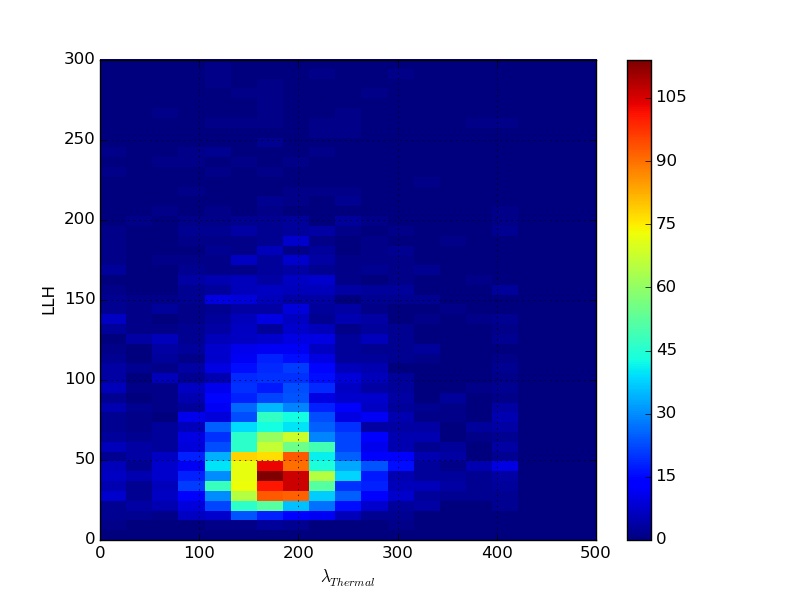
\includegraphics[width=0.5\linewidth]{llh_vs_thermal.png} &
	 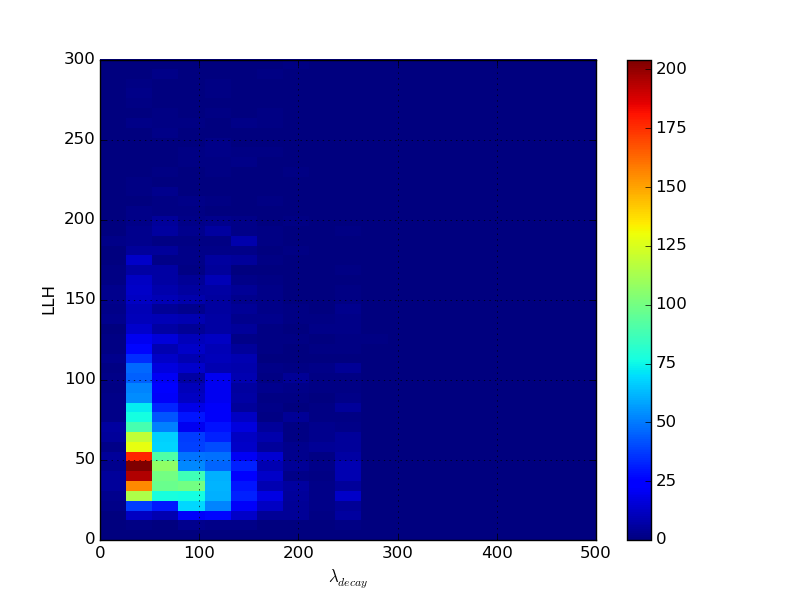
\includegraphics[width=0.5\linewidth]{llh_vs_decay.png} \\
 	 
 	 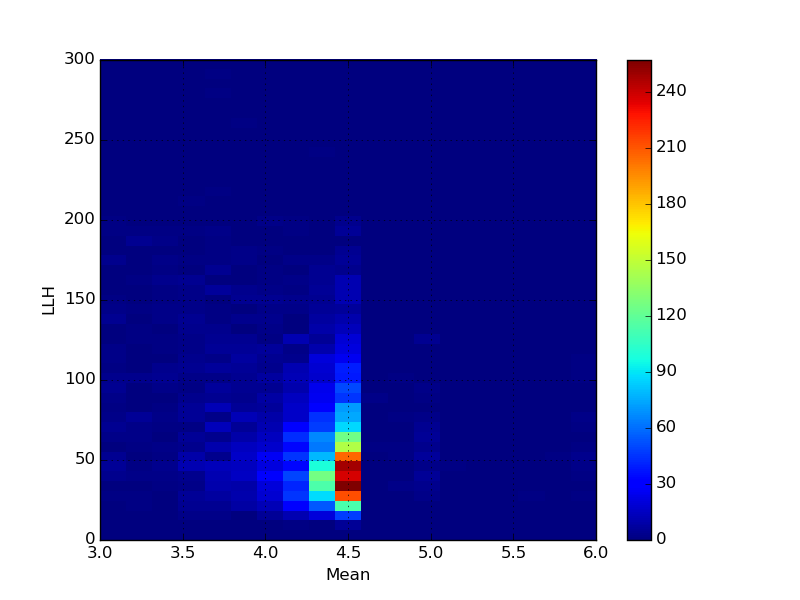
\includegraphics[width=0.5\linewidth]{llh_vs_mean.png}  &
	 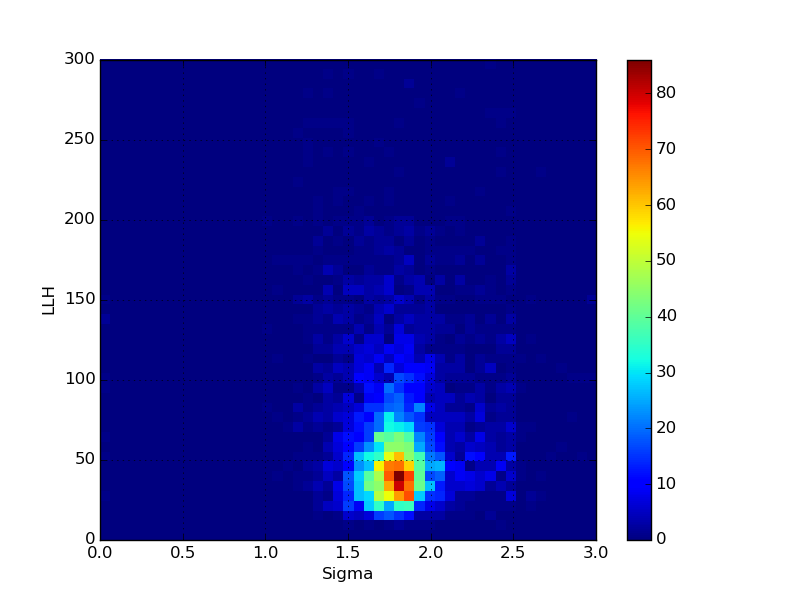
\includegraphics[width=0.5\linewidth]{llh_vs_sigma.png} \\

	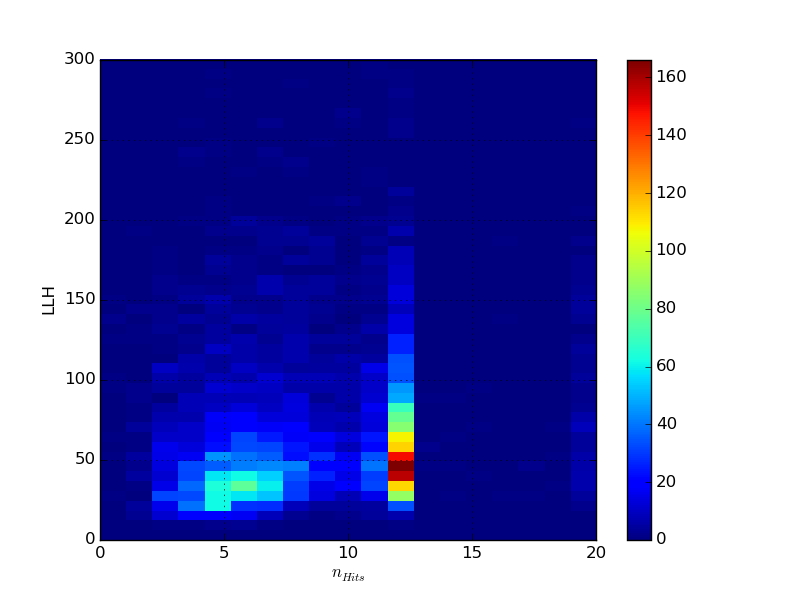
\includegraphics[width=0.5\linewidth]{llh_vs_nhits.png}  &
	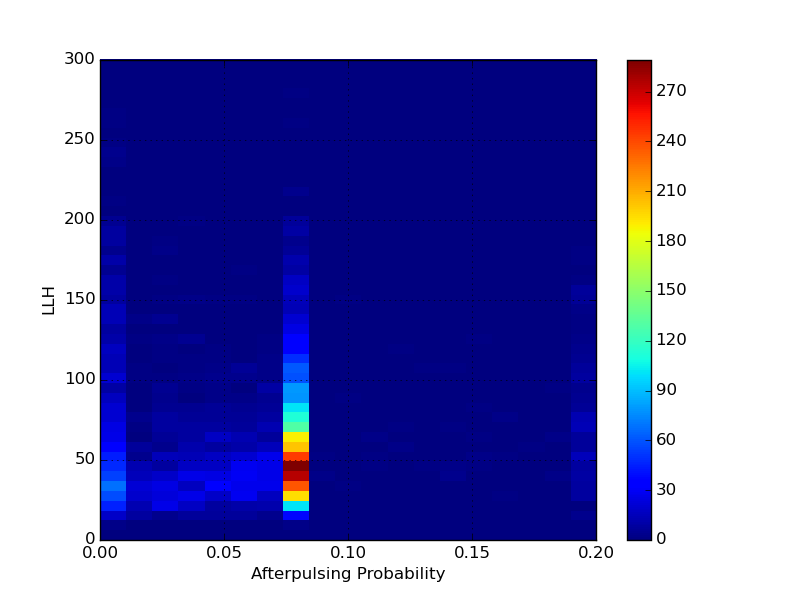
\includegraphics[width=0.5\linewidth]{llh_vs_afterpulsing.png} \\
\end{tabular}
\caption[Vuvzuela V2 likelihood values as a function of fit parameters ]The distributions of each new fit parameter in the Vuvuzela V2 model. The colorbar scale shows the number of DOMs in each bin.}
\label{fig:vuvuzela_params_vs_llh}
\end{figure}

The Vuvuzela V2 fits were checked after convergence in Figures~\ref{fig:vuvuzela_params_vs_llh} and \ref{fig:vuvuzela_params_occupancy}.
One notable feature is the number of DOMs with afterpulsing at the fitter boundary.
The likelihood values associated with these fits, however, appear to be consistent with other fits.
Due to a planned overhaul of the afterpulsing simulation, the fit values of the afterpulsing probabilities have not been adopted for simulation.
Therefore, no further investigation of the probabilities has been persued.

\begin{figure}[h]
\centering
\begin{tabular}{cc}
  	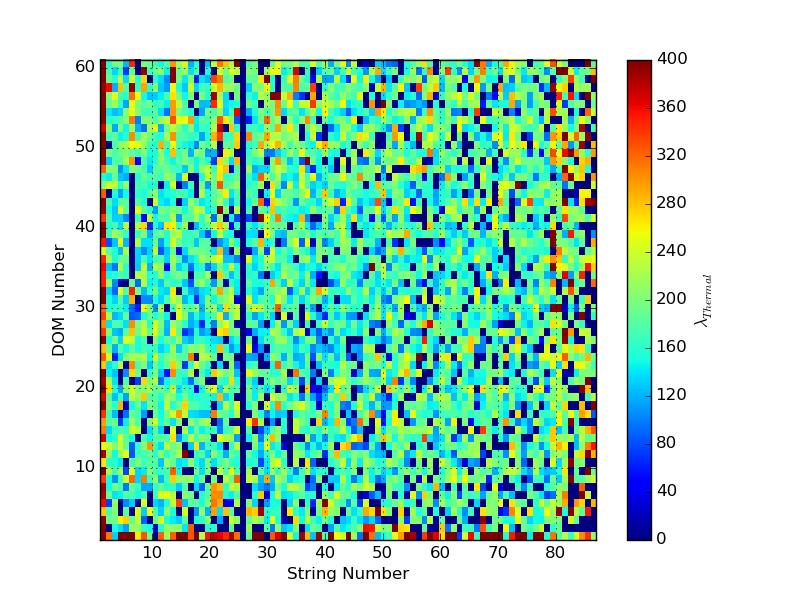
\includegraphics[width=0.5\linewidth]{thermal_occupancy.png} &
	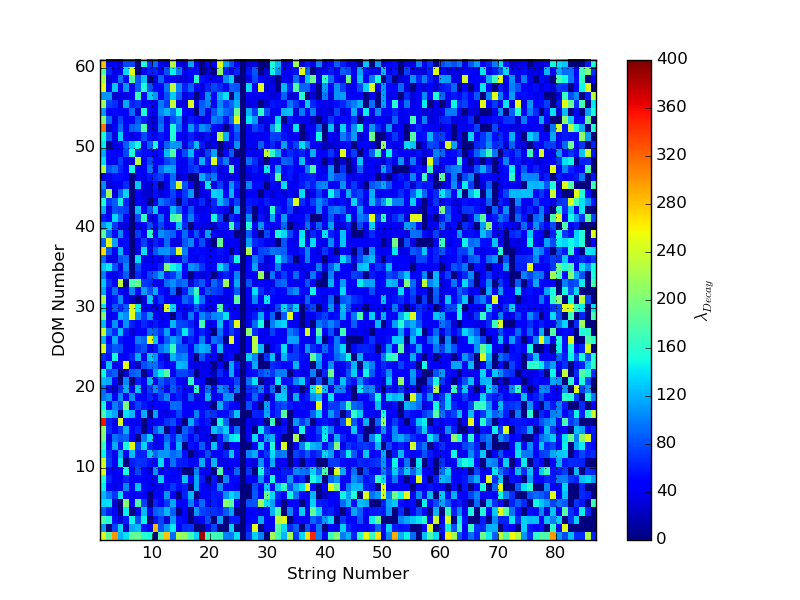
\includegraphics[width=0.5\linewidth]{decay_occupancy.png} \\

  	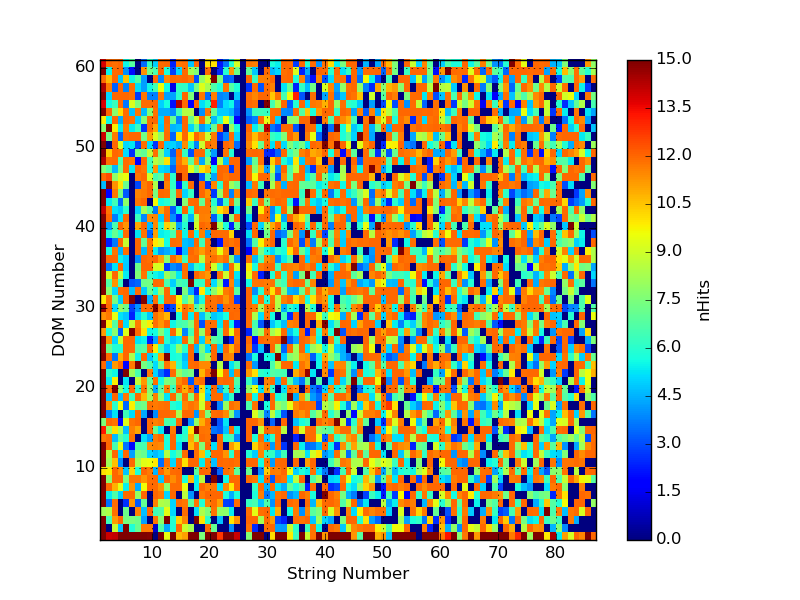
\includegraphics[width=0.5\linewidth]{nhits_occupancy.png} &
	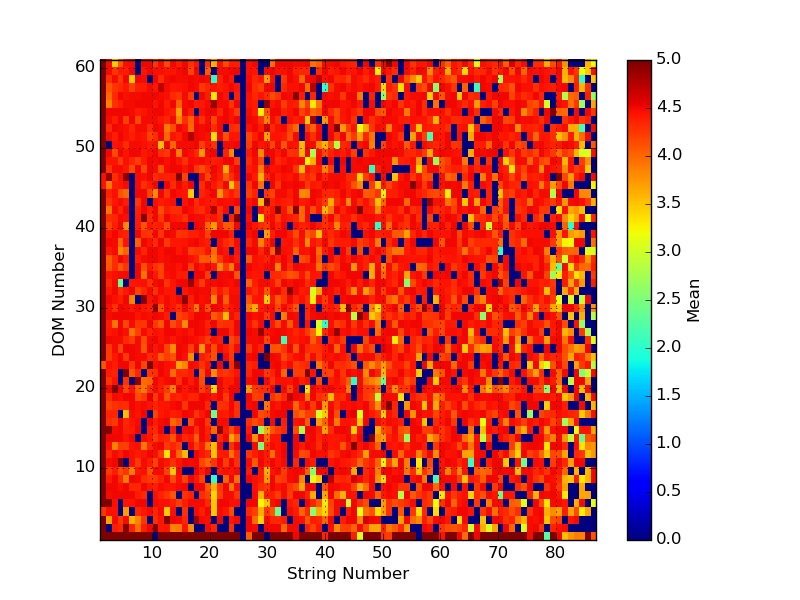
\includegraphics[width=0.5\linewidth]{mean_occupancy.png} \\

  	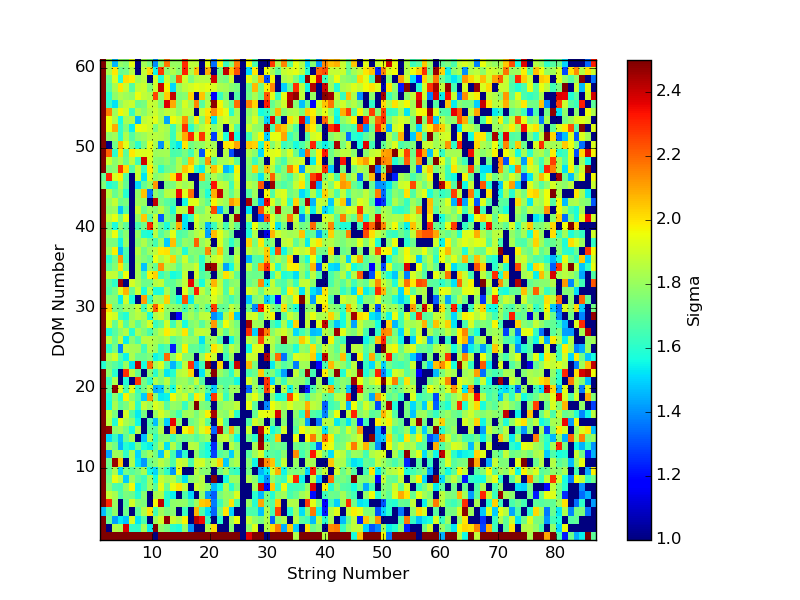
\includegraphics[width=0.5\linewidth]{sigma_occupancy.png} & 
  	\\
\end{tabular}	
\caption[Vuvuzela V2 fit parameters as a function of string and DOM number]{The distributions of each new fit parameter in the Vuvuzela V2 model as a function of the string and DOM number. Note that the top of the detector is at the bottom of this plot. No parameter appears to be correlated with depth. DOMs on string 25 are missing from the untriggered dataset used here and were not fit. In addition, DOMs which are disabled due to malfunction are also unavailable.}
\label{fig:vuvuzela_params_occupancy}
\end{figure}

The likelihood value was checked as a function of string and DOM number in Figure~\ref{fig:llh_vs_depth} to identify outliers.
The likelihood values appear to vary as a function of depth and shows at least two notable features: a "band" structure and an overall depth-dependence.
This was initially unexpected, given that the noise is an internal property of individual DOMs.

\begin{figure}
\centering
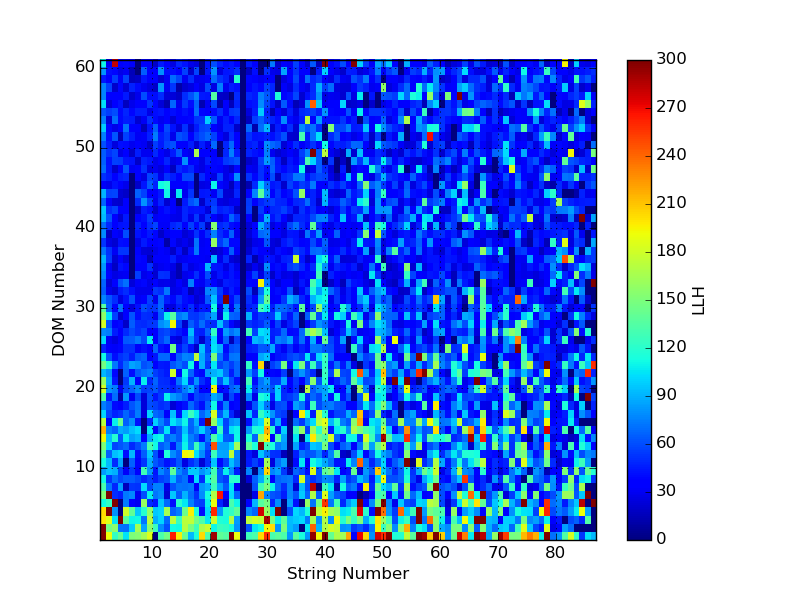
\includegraphics[width=0.9\textwidth]{llh.png} 
\caption[Vuvuzela V2 log-likelihood vs string and DOM number]{The log-likelihood as a function of string and DOM number for the Vuvuzela V2 fits. Note that DOM 1 is at the top of the detector and DOM 60 at the bottom. The likelihood value was expected to be independent of depth, but shows some structure. These structures are correlated with both the ice model and the muon flux.}
\label{fig:llh_vs_depth}
\end{figure}

It is worth noting that the noise measurements of each DOM are not fully independent due to the included simulated muons.
The fits use long-frame CORSIKA to model the effects of muons in the untriggered data from the detector.

This leads to two subtle limitations in the fitting process.
The long-frame CORSIKA is produced with a single flux model, in this case the Polygonato model used in CORSIKA \cite{Hoerandel-Polygonato}.
Disagreement between the Polygonato cosmic ray flux model and the data can lead to disagreement in the fitting of noise parameters.
The muon flux decreases with increasing depth, resulting in a lower muon contamination, and consequently smaller effects from mismodeling of the muon background, for deeper DOMs (higher DOM number). 

In addition, the long-frame CORSIKA implicitly assumes a single model of the ice for photon propagation.
Mismodeling of the scattering and absorption of photons from the CORSIKA simulation may also give rise to disagreement in the noise calibration.
While large-scale properties of the ice are believed to be well-reproduced by the chosen ice model, SpiceLea \cite{IceCube-SpiceLea}, there will inevitably be remaining disagreements.
The banding structure of Figure~\ref{fig:llh_vs_depth} corresponds to regions with low scattering and absorption at the top of the detector.

The uncertainties of the ice model and cosmic ray models together explain both features of Figure~\ref{fig:llh_vs_depth}.
In particular, the best fits occur where the DOM is either well-shielded from the Cherenkov light of muons due to either large overburden or strong absorption in the ice.
In both cases, the contamination from light due to muons in the fitted time and charge distributions will be small, leading to a more 'pure' noise distribution that is well-fit by the Vuvuzela V2 noise model.

The sensitivity of the noise calibration procedure to underlying assumptions of both the muon flux and the absorption properties in the detector imply that little further improvement is likely without additional work on one or both issues.
Simulation of long-frame CORSIKA is not possible with newer flux models at this time.
As the primary uncertainty affecting the goodness-of-fit appears to be related to the muons themselves, merely updating to a newer model of the ice is  unlikely to significantly improve the current fit parameters.

The newly calibrated low-dt Vuvuzela was provided to the IceCube simulation group in January of 2015 and quickly integrated into the low-energy simulation chain.
New neutrino, muon, and accidental noise trigger simulations were produced soon thereafter.
The updated noise model shows significantly better agreement in both the total charge distribution and the number of hit DOMs for both HLC and SLC+HLC hits.
The rate of accidental triggers improved relative to previous calibrations, with the remaining rate disagreement reduced from 50\% to approximately 15\%.
Negligible effect was observed in the low-energy neutrino events at final level for existing samples.

